% Options for packages loaded elsewhere
\PassOptionsToPackage{unicode}{hyperref}
\PassOptionsToPackage{hyphens}{url}
%
\documentclass[
]{article}
\usepackage{amsmath,amssymb}
\usepackage{iftex}
\ifPDFTeX
  \usepackage[T1]{fontenc}
  \usepackage[utf8]{inputenc}
  \usepackage{textcomp} % provide euro and other symbols
\else % if luatex or xetex
  \usepackage{unicode-math} % this also loads fontspec
  \defaultfontfeatures{Scale=MatchLowercase}
  \defaultfontfeatures[\rmfamily]{Ligatures=TeX,Scale=1}
\fi
\usepackage{lmodern}
\ifPDFTeX\else
  % xetex/luatex font selection
\fi
% Use upquote if available, for straight quotes in verbatim environments
\IfFileExists{upquote.sty}{\usepackage{upquote}}{}
\IfFileExists{microtype.sty}{% use microtype if available
  \usepackage[]{microtype}
  \UseMicrotypeSet[protrusion]{basicmath} % disable protrusion for tt fonts
}{}
\makeatletter
\@ifundefined{KOMAClassName}{% if non-KOMA class
  \IfFileExists{parskip.sty}{%
    \usepackage{parskip}
  }{% else
    \setlength{\parindent}{0pt}
    \setlength{\parskip}{6pt plus 2pt minus 1pt}}
}{% if KOMA class
  \KOMAoptions{parskip=half}}
\makeatother
\usepackage{xcolor}
\usepackage{graphicx}
\usepackage{subcaption}
\makeatletter
\def\maxwidth{\ifdim\Gin@nat@width>\linewidth\linewidth\else\Gin@nat@width\fi}
\def\maxheight{\ifdim\Gin@nat@height>\textheight\textheight\else\Gin@nat@height\fi}
\makeatother
% Scale images if necessary, so that they will not overflow the page
% margins by default, and it is still possible to overwrite the defaults
% using explicit options in \includegraphics[width, height, ...]{}
\setkeys{Gin}{width=\maxwidth,height=\maxheight,keepaspectratio}
% Set default figure placement to htbp
\makeatletter
\def\fps@figure{htbp}
\makeatother
\setlength{\emergencystretch}{3em} % prevent overfull lines
\providecommand{\tightlist}{%
  \setlength{\itemsep}{0pt}\setlength{\parskip}{0pt}}
\setcounter{secnumdepth}{-\maxdimen} % remove section numbering
\ifLuaTeX
  \usepackage{selnolig}  % disable illegal ligatures
\fi
\IfFileExists{bookmark.sty}{\usepackage{bookmark}}{\usepackage{hyperref}}
\IfFileExists{xurl.sty}{\usepackage{xurl}}{} % add URL line breaks if available
\urlstyle{same}
\hypersetup{
  pdftitle={Comparazione tra algoritmi di ordinamento Insertion Sort, Quick Sort},
  pdfauthor={Leonardo Toccafondi},
  hidelinks,
  pdfcreator={LaTeX via pandoc}}

\title{Comparazione tra algoritmi di ordinamento Insertion Sort, Quick
Sort}
\author{Leonardo Toccafondi}
\date{Febbraio, 2023}

\begin{document}
\maketitle

\hypertarget{introduzione}{%
\section{Introduzione}\label{introduzione}}

Una delle classi di problemi più studiate nel campo dell'informatica
sono i problemi di ordinamento. Essi possono essere descritti nel
seguente modo:

\begin{quote}
\emph{A partire da una sequenza di dati \(S = \{x_1, \dotsc, x_n\}\) in
ingresso trovare una permutazione
\(S^{\prime} = > > \{x_1^{\prime}, \dotsc , x_n^{\prime}\}\) di essa
tale che
\(x_1^{\prime} \leq x_2^{\prime} \leq \dotsc \leq x_n^\prime\).}
\end{quote}

Per la loro risoluzione sono stati pensati numerosi algoritmi di
ordinamento: ogni implementazione differisce soprattutto per i campi di
applicazione e per il comportamento rispetto a certe sequenze di
ingresso. Per valutare quale sia meglio usare è quindi necessario
valutare la loro efficienza, ovvero quanto tempo impiegano ad essere
eseguiti su insiemi di dati particolari e con dimensione sempre
crescente. In questa relazione saranno analizzate le differenze, in
senso di \emph{complessità temporale}, di due algoritmi di ordinamento:
\textbf{Quick Sort} e \textbf{Insertion Sort}. In particolare saranno
analizzati i loro andamenti temporali all'aumentare del numero di
elementi delle liste da ordinare.

\hypertarget{teoria}{%
\section{Teoria}\label{teoria}}

\hypertarget{insertion-sort}{%
\subsubsection{Insertion sort}\label{insertion-sort}}

\hypertarget{descrizione-dellalgoritmo}{%
\paragraph{Descrizione dell'algoritmo}\label{descrizione-dellalgoritmo}}

Insertion sort è un algoritmo di ordinamento sul posto che prende prende
in ingresso una sequenza di \(n\) numeri memorizzati in un array A, e
restituisce una loro permutazione
\(\{A'_{1}, A'_{2}, \dotsc , A'_{n} \}\) ordinata.

Il funzionamento è simile a come si ordinano le carte in mano: alla
j-esima iterazione l'algoritmo sposta'' la chiave indietro nell'array,
finché non si trova n elemento minore oppure si è arrivati alla fine
dell'array. In questo modo la chiave viene inserita nella posizione
corretta (j+1-esima posizione). Quindi ad ogni iterazione il sottoarray
\(A[1, \dotsc, j-1]\) è formato da elementi che originariamente erano in
\(A[1, \dotsc, j-1]\), ma adesso sono \textbf{ordinati}.

Insertion sort è un algoritmo \textbf{stabile}, in quanto ordina gli
elementi uguali nello stesso ordine in cui appaiono nell'input. Inoltre
ordina sul posto, senza l'ausilio di liste ulteriori. Inoltre è
\textbf{adattivo}, in quanto è efficiente per insiemi di dati che sono
già sostanzialmente ordinati.

\hypertarget{prestazioni-attese}{%
\paragraph{Prestazioni attese}\label{prestazioni-attese}}

Per definire le prestazioni attese di Insertion sort è necessario
analizzare il suo costo. Per come è strutturato l'algoritmo, la
complessità dipende sia dalla dimensione dell'input, sia da come sono
ordinati i dati. Quindi, a parità di quantità di dati, l'algoritmo può
essere più o meno veloce a seconda della loro disposizione nella
sequenza. Per questo motivo si distinguono tre casi:

\begin{itemize}
\item
  \textbf{Caso migliore:} gli elementi sono già ordinati. In questo caso
  il costo è \(\Theta(n)\);
\item
  \textbf{Caso peggiore:} gli elementi sono ordinati al contrario. In
  questo caso il costo è \(\Theta(n^{2})\);
\item
  \textbf{Caso medio:} gli elementi sono ordinati in modo casuale.
  Questo caso è simile al caso peggiore ed ha la stessa complessità
\end{itemize}

Rispetto ad un algoritmo \emph{divide-et-impera} performa peggio per set
di dati molto grandi, mentre ha ottime prestazioni per set di dati più
ridotti

\hypertarget{quick-sort}{%
\subsubsection{Quick Sort}\label{quick-sort}}

\hypertarget{descrizione-dellalgoritmo-1}{%
\paragraph{Descrizione
dell'algoritmo}\label{descrizione-dellalgoritmo-1}}

Quick sort è un algoritmo di ordinamento sul posto ma, a differenza di
insertion sort, è ricorsivo e si basa sul principio \emph{divide et
impera}. Per ordinare un array \(A[p,\_\_\_, r]\):

\begin{itemize}
\item
  \textbf{Divide:} partiziona l'array A in due sottoarray
  \(A[p,\dotsc, q-1]\) e \(A[q+1,\dotsc, r]\) tali che ogni elemento del
  primo sottoarray è minore di q (o uguale) e ogni elemento del secondo
  sottoarray è maggiore di q (o uguale). L'elemento \(A[q]\) prende il
  nome di \emph{pivot}.
\item
  \textbf{Impera:} ordina i due sottoarray con chiamate ricorsive a se
  stessa.
\item
  \textbf{Combina:} combina i due sottoarray ordinati per restituire
  l'array \(A[p,\dotsc, r]\) ordinato.
\end{itemize}

\hypertarget{prestazioni-attese-1}{%
\paragraph{Prestazioni attese}\label{prestazioni-attese-1}}

Il tempo di esecuzione del Quick sort dipende dal partizionamento dei
sottoarray, ovvero se questi ultimi sono bilanciati o sbilanciati:

\begin{itemize}
\item
  \textbf{Partizionamento nel caso peggiore:} si ha quando l'array è già
  ordinato. Infatti in questo caso la funzione partition divide il
  problema in due sottoproblemi, uno di grandezza \(n - 1\) e l'altro di
  grandezza \(0\). Il costo è, quindi, \(\Theta(n^{2})\).
\item
  \textbf{Partizionamento nel caso migliore:} si ha quando, ad ogni
  iterazione, il pivot scelto è l'elemento che divide l'array in due
  sottoproblemi di dimensione uguale. Quindi ciascun sottoarray avrà
  dimensione \(\dfrac{n}{2}\). In questo caso il costo è
  \(\mathcal{O}(n\log{}n)\)
\item
  \textbf{Partizionamento nel caso medio:} i due sottoarray sono divisi
  in modo casuale. Questo caso è simile al caso migliore ed ha la stessa
  complessità.
\end{itemize}

\hypertarget{esperimenti-svolti}{%
\section{Esperimenti svolti}\label{esperimenti-svolti}}

In questa relazione, sono stati misurati i tempi di esecuzione degli
algoritmi di ordinamento all'aumentare del numero di elementi nella
lista da passare agli stessi. Gli esperimenti sono stati fatti su un
numero massimo di nodi pari a 10000, andando a misurare sia i tempi di
esecuzione per array già ordinati (sia in senso crescente che
decrescente), sia per un array randomizzato (viene passato lo stesso in
tutti e due i casi). Le misurazioni, in questo caso, avvengono ogni
incremento di 100 nodi.

I tempi di esecuzione sono stati salvati in delle liste separate, una
per ciascun algoritmo, inserendo successivamente i valori in una
tabella, poi salvata in formato txt. Infine questi valori sono stati
utilizzati per creare grafici rappresentanti andamenti temporali.

Viene distinto il caso ordinato, da quello non ordinato, con un
controllo sulla variabile booleana \emph{shuffle}, grazie alla quale il
programma sa se randomizzare o meno i valori della lista da ordinare, se
questa è pari a True. Altrimenti, l'input non viene randomizzato e avrò
come risultato il caso migliore di Insertion sort. Inoltre, con un altra
variabile booleana \emph{rev} è possibile invertire l'ordine dell'array
ordinato, ottenendo il caso peggiore di Insertion sort.

\hypertarget{implementazione-pratica}{%
\section{Implementazione pratica}\label{implementazione-pratica}}

Il programma è suddiviso in più file:

\begin{itemize}
\tightlist
\item
  insertion\_sort.py, quick\_sort.py, i quali si occupano
  dell'implementazione degli algoritmi di ordinamento da testare;
\item
  test.py: è il programma principale, si occupa del test degli algoritmi
  e della creazione dei grafici.
\end{itemize}

\hypertarget{ambiente-di-test}{%
\paragraph{Ambiente di test}\label{ambiente-di-test}}

L'esperimento è stato svolto su un computer con le seguenti
caratteristiche:

\begin{itemize}
\item
  Sistema operativo: Linux Mint 21.1 con kernel 5.15
\item
  CPU: Inter Core i7-9750H
\item
  RAM: 16 GB
\item
  Interprete Python: conda 22.11.1 e python v 3.10
\item
  IDE: Pycharm Community Edition 2022.3.2
\end{itemize}

\hypertarget{risultati}{%
\section{Risultati}\label{risultati}}

\begin{table}[!h]
    \begin{center}
        \begin{tabular}{|c|c|c|}
            \hline \hline Numero di valori & Insertion Sort & Quick Sort \\
            \hline \hline 100              & 0              & $0.0016$   \\
            \hline 1000                    & $0.0002$       & $0.1488$   \\
            \hline 2000                    & $0.0004$       & $0.5915$   \\
            \hline 3000                    & $0.0007$       & $1.4455$   \\
            \hline 4000                    & $0.0009$       & $2.3383$   \\
            \hline 5000                    & $0.0011$       & $3.6908$   \\
            \hline 6000                    & $0.0013$       & $5.3176$   \\
            \hline 7000                    & $0.002$        & $7.4722$   \\
            \hline 8000                    & $0.0018$       & $9.4267$   \\
            \hline 10000                   & $0.0021$       & $11.9687$  \\
            \hline \hline
        \end{tabular}
    \end{center}
    \caption{Confronto tempi array ordinato}
\end{table}

\begin{table}[!h]
    \begin{center}
        \begin{tabular}{|c|c|c|}
            \hline Numero di valori & Insertion Sort & Quick Sort \\
            \hline \hline 100       & $0.001$        & $0.0009$   \\
            \hline 1000             & $0.1024$       & $0.0929$   \\
            \hline 2000             & $0.4048$       & $0.3731$   \\
            \hline 3000             & $0.918$        & $0.847$    \\
            \hline 4000             & $1.6281$       & $1.508$    \\
            \hline 5000             & $2.587$        & $2.3577$   \\
            \hline 6000             & $3.7017$       & $3.3955$   \\
            \hline 7000             & $5.026$        & $4.6437$   \\
            \hline 8000             & $6.5952$       & $6.0721$   \\
            \hline 10000            & $10.2898$      & $7.6807$   \\
            \hline \hline
        \end{tabular}
    \end{center}
    \caption{Confronto tempi array ordinato in ordine decrescente}
\end{table}

\begin{table}[h!]
    \begin{center}
        \begin{tabular}{|c|c|c|}
            \hline \hline Numero di valori & Insertion Sort & Quick Sort \\
            \hline \hline 100              & $0.0005$       & $0.0002$   \\
            \hline 1000                    & $0.051$        & $0.0024$   \\
            \hline 2000                    & $0.2088$       & $0.0064$   \\
            \hline 3000                    & $0.4531$       & $0.0085$   \\
            \hline 4000                    & $0.8249$       & $0.0123$   \\
            \hline 5000                    & $1.2882$       & $0.0153$   \\
            \hline 6000                    & $1.8727$       & $0.0197$   \\
            \hline 7000                    & $2.5031$       & $0.025$    \\
            \hline 8000                    & $3.2852$       & $0.0254$   \\
            \hline 9000                    & $4.1418$       & $0.0293$   \\
            \hline 10000                   & $5.073$        & 0341       \\
            \hline \hline
        \end{tabular}
    \end{center}
    \caption{Confronto tempi array randomizzato}
\end{table}
\newpage
\begin{figure}[h!]
    \centering
    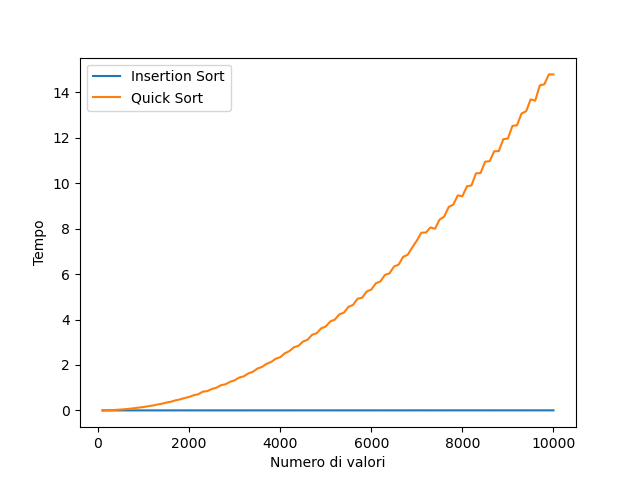
\includegraphics{../img/ord/ord_comparison10000.png}
    \caption{Confronto tempi con array ordinato}
\end{figure}

\begin{figure}[h!]
    \centering
    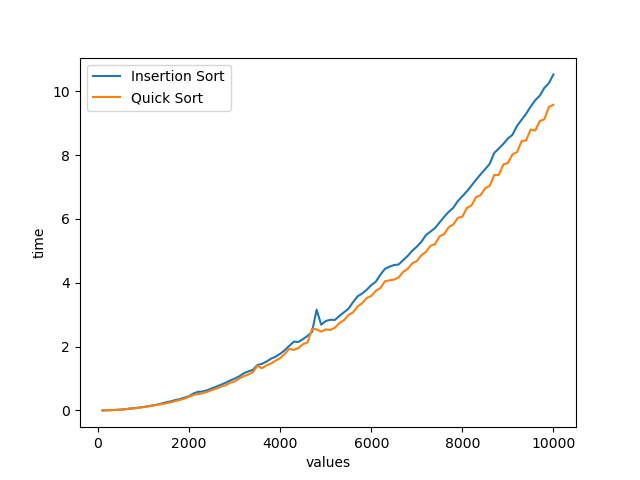
\includegraphics{../img/ord_rev/ord_rev_comparison10000.png}
    \caption{Confronto tempi con array ordinato in ordine decrescente}
\end{figure}

\newpage

\begin{figure}[h!]
    \centering
    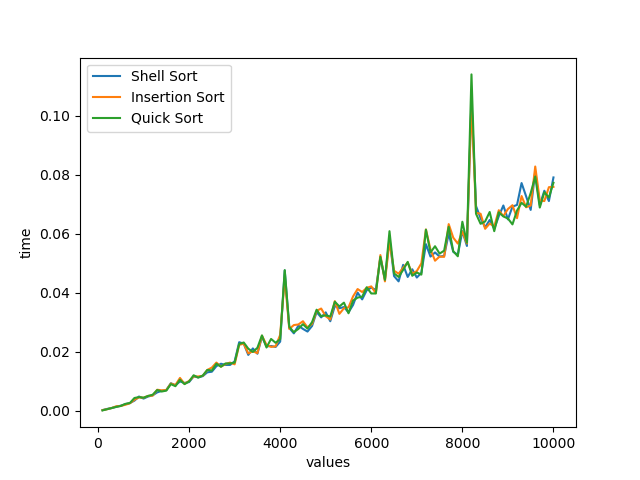
\includegraphics{../img/rand/rand_comparison10000.png}
    \caption{Confronto tempi con array randomizzato}
    \label{fig:3}
\end{figure}
\newpage



\
\
\

\
\newpage
\newpage
\hypertarget{conclusioni}{%


    \section{Conclusioni}\label{conclusioni}}

Come si evince dai grafi, le performance attese da entrambi gli
algoritmi di ordinamento sono state rispettate: infatti, insertion sort
risulta essere più efficace di Quick sort soltanto nel caso in cui
l'array da ordinare sia già ordinato. In questo caso quick sort è nel
suo caso peggiore.

Osservando la figura 2, che rappresenta i tempi di esecuzione nel caso
dell'array ordinato in senso decrescente (quindi per il caso peggiore di
insertion sort), si può vedere come quick sort si avvicini molto ai
tempi di insertion sort, pur rimanendo inferiore.

In figura 3, che raffigura i tempi di esecuzione per il caso medio di
quick sort, è evidente la maggiore efficienza di quick sort, che arriva
ad essere centinaia di volte più veloce di insertion sort.

In conclusione quick sort è l'algoritmo preferibile nella quasi totalità delle
applicazioni, nonostante questo insertion sort ha comunque degli
usi reali. Un esempio può essere un insieme di dati
dinamico, in cui vengono aggiunti spesso degli elementi che non
modificano troppo la struttura dell'insieme. In un caso come questo
abbiamo un insieme quasi sempre ordinato a meno di qualche elemento,
caso in cui insertion sort ha un comportamento quasi lineare.

\end{document}
